% !TEX program = pdflatex
% !TEX options = --shell-escape -synctex=1 -interaction=nonstopmode -file-line-error "%DOC%"
\documentclass[notitlepage]{article}
\usepackage{float}
\usepackage{verbatim}
\usepackage{amsmath}
\usepackage{listings}
\usepackage{bm}
\usepackage{graphicx}
\usepackage{booktabs}
\usepackage{color,xcolor}
\usepackage{enumerate}
\usepackage{minted}
\usepackage{caption}
\usepackage{subcaption}
\usepackage{amssymb}
\usepackage{hyperref}

\title{Poisson-FBMP Note}
\date{}

\definecolor{dkgreen}{rgb}{0,0.6,0}
\definecolor{gray}{rgb}{0.5,0.5,0.5}
\definecolor{mauve}{rgb}{0.58,0,0.82}
\lstset{
    language=python,
    basicstyle=\footnotesize,
    numbers=left,
    numberstyle=\tiny\color{gray},
    stepnumber=2,
    numbersep=5pt,
    backgroundcolor=\color{white},
    showspaces=false,
    showstringspaces=false,
    showtabs=false,
    frame=single,
    rulecolor=\color{black},
    tabsize=2,
    captionpos=b,
    breaklines=true,
    breakatwhitespace=false,
    title=\lstname,
    keywordstyle=\color{blue},
    commentstyle=\color{dkgreen},
    stringstyle=\color{mauve},
    escapeinside={\%*}{*)},
    morekeywords={*,...}
}

\begin{document}
\newcommand{\ud}{\mathrm{d}}

\maketitle
\tableofcontents

\section{Phenomenon}

\subsection{P-FBMP with magic time bin}

\begin{lstlisting}
mu_t = abs(wave.sum() / gmu)
if Tau > 10:
    n = min(math.ceil(20 / mu_t), 5)
else:
    n = min(math.ceil(4 / mu_t), 3)
A, wave_r, tlist, t0_t, t0_delta, cha, left_wave, right_wave = wff.initial_params(wave[::wff.nshannon], spe_pre[ent[i]['ChannelID']], Mu, Tau, Sigma, gmu, Thres['lucyddm'], p, nsp, nstd, is_t0=True, is_delta=False, n=n, nshannon=1)
mu_t = abs(wave_r.sum() / gmu)
def optit0mu(t0, mu, n, xmmse_star, psy_star, c_star, la):
    ys = np.log(psy_star) - np.log(poisson.pmf(c_star, la)).sum(axis=1)
    ys = np.exp(ys - ys.max()) / np.sum(np.exp(ys - ys.max()))
    t0list = np.arange(t0 - 3 * Sigma, t0 + 3 * Sigma + 1e-6, 0.2)
    mulist = np.arange(max(1e-8, mu - 3 * np.sqrt(mu)), mu + 3 * np.sqrt(mu), 0.1)
    b_mu = [max(1e-8, mu - 5 * np.sqrt(mu)), mu + 5 * np.sqrt(mu)]
    tlist_pan = np.sort(np.unique(np.hstack(np.arange(0, window)[:, None] + np.arange(0, 1, 1 / n))))
    As = np.zeros((len(xmmse_star), len(tlist_pan)))
    As[:, np.isin(tlist_pan, tlist)] = c_star
    assert sum(np.sum(As, axis=0) > 0) > 0

    def likelihood(x):
        a = x[0] * wff.convolve_exp_norm(tlist_pan - x[1], Tau, Sigma) / n + 1e-8 # use tlist_pan not tlist
        li = -special.logsumexp(np.log(poisson.pmf(As, a)).sum(axis=1), b=ys)
        return li

    likemu = np.array([likelihood([mulist[j], t0]) for j in range(len(mulist))])
    liket0 = np.array([likelihood([mu, t0list[j]]) for j in range(len(t0list))])
    mu, t0 = opti.fmin_l_bfgs_b(likelihood, x0=[mulist[likemu.argmin()], t0list[liket0.argmin()]], approx_grad=True, bounds=[b_mu, b_t0], maxfun=50000)[0]
    return mu, t0

truth = pelist[pelist['TriggerNo'] == ent[i]['TriggerNo']]
time_fbmp_start = time.time()
factor = np.sqrt(np.diag(np.matmul(A.T, A)).mean())
A = np.matmul(A, np.diag(1. / np.sqrt(np.diag(np.matmul(A.T, A)))))
la = mu_t * wff.convolve_exp_norm(tlist - t0_t, Tau, Sigma) / n + 1e-8
xmmse, xmmse_star, psy_star, nu_star, nu_star_bk, T_star, d_tot_i, d_max_i, num_i = wff.fbmpr_fxn_reduced(wave_r, A, la, spe_pre[cid]['std'] ** 2, (gsigma * factor / gmu) ** 2, factor, len(la), stop=5, truth=truth, i=i, left=left_wave, right=right_wave, tlist=tlist, gmu=gmu, para=p)
time_fbmp = time_fbmp + time.time() - time_fbmp_start
c_star = np.zeros_like(xmmse_star).astype(int)
for k in range(len(T_star)):
    t, c = np.unique(T_star[k][xmmse_star[k][T_star[k]] > 0], return_counts=True)
    c_star[k, t] = c
maxindex = 0

xmmse_most = xmmse_star[maxindex]
pet = np.repeat(tlist[xmmse_most > 0], c_star[maxindex][xmmse_most > 0])
cha = np.repeat(xmmse_most[xmmse_most > 0] / factor / c_star[maxindex][xmmse_most > 0], c_star[maxindex][xmmse_most > 0])

mu, t0 = optit0mu(t0_t, mu_t, n, xmmse_star, psy_star, c_star, la)
mu_i, t0_i = optit0mu(t0_t, mu_t, n, xmmse_most[None, :], np.array([1]), c_star[maxindex][None, :], la)
\end{lstlisting}

Motivation: demonstrate magic time binning on $\mu$ bias

Progress: magic time bin is
\begin{lstlisting}
mu_t = abs(wave.sum() / gmu)
if Tau > 10:
    n = min(math.ceil(20 / mu_t), 5)
else:
    n = min(math.ceil(4 / mu_t), 3)
\end{lstlisting}

Result: relative $\mu$ bias are less than $2.5\%$

\begin{figure}[H]
    \centering
    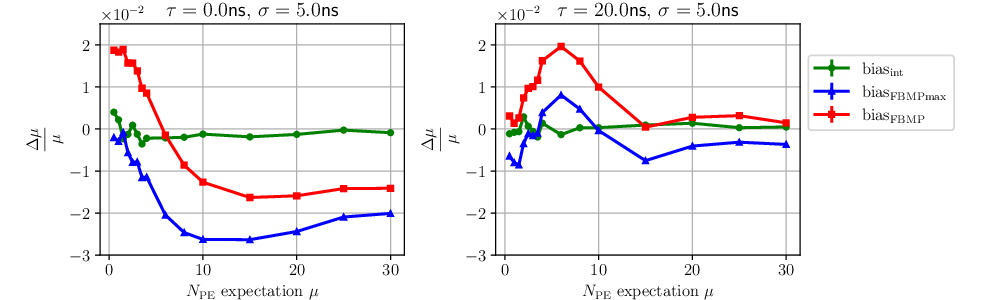
\includegraphics[width=\textwidth]{vs-biasmu-magic.png}
\end{figure}

\subsection{P-FBMP only fitting}

\begin{lstlisting}
def optit0mu(t0, mu, n, xmmse_star, psy_star, c_star, la):
    ys = np.log(psy_star) - np.log(poisson.pmf(c_star, la)).sum(axis=1)
    ys = np.exp(ys - ys.max()) / np.sum(np.exp(ys - ys.max()))
    t0list = np.arange(t0 - 3 * Sigma, t0 + 3 * Sigma + 1e-6, 0.2)
    mulist = np.arange(max(1e-8, mu - 3 * np.sqrt(mu)), mu + 3 * np.sqrt(mu), 0.1)
    b_mu = [max(1e-8, mu - 5 * np.sqrt(mu)), mu + 5 * np.sqrt(mu)]
    tlist_pan = np.sort(np.unique(np.concatenate([np.unique(np.hstack(np.arange(1, window-1)[:, None] + np.arange(0, 1, 1 / n))), tlist])))
    As = np.zeros((len(xmmse_star), len(tlist_pan)))
    As[:, np.isin(tlist_pan, tlist)] = c_star
    tlist_edge = np.concatenate([[tlist_pan[0] - np.diff(tlist_pan)[0] / 2], (tlist_pan[1:] + tlist_pan[:-1]) / 2, [tlist_pan[-1] + np.diff(tlist_pan)[-1] / 2]])
    diff = np.diff(tlist_edge)
    assert As.sum() == c_star.sum()
    assert sum(np.sum(As, axis=0) > 0) > 0

    def likelihood(x):
        a = x[0] * wff.convolve_exp_norm(tlist_pan - x[1], Tau, Sigma) * diff + 1e-8 # use tlist_pan not tlist
        li = -special.logsumexp(np.log(poisson.pmf(As, a)).sum(axis=1), b=ys)
        return li

    likemu = np.array([likelihood([mulist[j], t0]) for j in range(len(mulist))])
    liket0 = np.array([likelihood([mu, t0list[j]]) for j in range(len(t0list))])
    mu, t0 = opti.fmin_l_bfgs_b(likelihood, x0=[mulist[likemu.argmin()], t0list[liket0.argmin()]], approx_grad=True, bounds=[b_mu, b_t0], maxfun=50000)[0]
    return mu, t0

truth = pelist[pelist['TriggerNo'] == ent[i]['TriggerNo']]

tlist = truth['HitPosInWindow'][truth['HitPosInWindow'] < right_wave - 1]
if len(tlist) == 1:
    tlist_edge = np.array([tlist[0] - 0.5, tlist[0] + 0.5])
else:
    tlist_edge = np.concatenate([[tlist[0] - np.diff(tlist)[0] / 2], (tlist[1:] + tlist[:-1]) / 2, [tlist[-1] + np.diff(tlist)[-1] / 2]])
t_auto = (np.arange(left_wave, right_wave) / wff.nshannon)[:, None] - tlist
A = p[2] * np.exp(-1 / 2 * (np.log((t_auto + np.abs(t_auto)) / p[0] / 2) / p[1]) ** 2)

t0_t = t0_truth[i]['T0']
mu_t = len(truth)
la = mu_t * np.array([integrate.quad(lambda t : wff.convolve_exp_norm(t - t0_t, Tau, Sigma), tlist_edge[i], tlist_edge[i+1])[0] for i in range(len(tlist))]) + 1e-8

c_star_truth = np.ones_like(tlist)
wav_ans = np.sum([np.where(pp > truth['HitPosInWindow'][j], wff.spe(pp - truth['HitPosInWindow'][j], tau=p[0], sigma=p[1], A=p[2]) * truth['Charge'][j] / gmu, 0) for j in range(len(truth))], axis=0)

mu, t0 = optit0mu(t0_t, mu_t, n, np.empty(len(la))[None, :], np.array([1]), c_star_truth[None, :], la)
\end{lstlisting}

Motivation: to validate fitting process

Progress: Use true \texttt{HitPosInWindow} as \texttt{tlist}, true \texttt{T0} as \texttt{t0\_t}, length of \texttt{HitPosInWindow} as \texttt{mu\_t}. Without FBMP RGS, directly \textbf{fit} $\mu$ and $t_0$. 

Result: fitting process is not related to bias of $\mu$. 

\begin{figure}[H]
    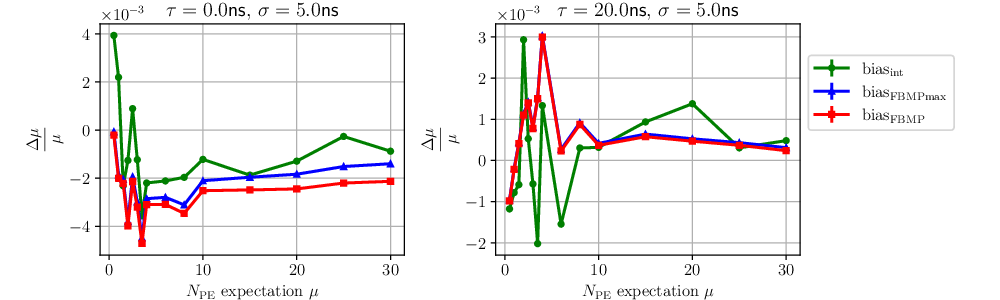
\includegraphics[width=\textwidth]{vs-biasmu-trufit.png}
\end{figure}

\subsection{P-FBMP with truth prior}

\begin{lstlisting}
tlist = truth['HitPosInWindow'][truth['HitPosInWindow'] < right_wave - 1]
if len(tlist) == 1:
    tlist_edge = np.array([tlist[0] - 0.5, tlist[0] + 0.5])
else:
    tlist_edge = np.concatenate([[tlist[0] - np.diff(tlist)[0] / 2], (tlist[1:] + tlist[:-1]) / 2, [tlist[-1] + np.diff(tlist)[-1] / 2]])
t_auto = (np.arange(left_wave, right_wave) / wff.nshannon)[:, None] - tlist
A = p[2] * np.exp(-1 / 2 * (np.log((t_auto + np.abs(t_auto)) / p[0] / 2) / p[1]) ** 2)
t0_t = t0_truth[i]['T0']
mu_t = len(truth)
factor = np.sqrt(np.diag(np.matmul(A.T, A)))
A = np.matmul(A, np.diag(1. / np.sqrt(np.diag(np.matmul(A.T, A)))))
la = mu_t * np.array([integrate.quad(lambda t : wff.convolve_exp_norm(t - t0_t, Tau, Sigma), tlist_edge[i], tlist_edge[i+1])[0] for i in range(len(tlist))]) + 1e-8
xmmse, xmmse_star, psy_star, nu_star, nu_star_bk, T_star, d_tot_i, d_max_i, num_i = wff.fbmpr_fxn_reduced(wave_r, A, la, spe_pre[cid]['std'] ** 2, (gsigma * factor / gmu) ** 2, factor, len(la), stop=5, truth=truth, i=i, left=left_wave, right=right_wave, tlist=tlist, gmu=gmu, para=p)
c_star = np.zeros_like(xmmse_star).astype(int)
for k in range(len(T_star)):
    t, c = np.unique(T_star[k][xmmse_star[k][T_star[k]] > 0], return_counts=True)
    c_star[k, t] = c
mu = np.average(c_star.sum(axis=1), weights=psy_star)
t0 = t0_t
\end{lstlisting}

Motivation: to prove prior used in FBMP is not the origin of $\mu$ bias. 

Progress: Use true \texttt{HitPosInWindow} as \texttt{tlist}, true \texttt{T0} as \texttt{t0\_t}, length of \texttt{HitPosInWindow} as \texttt{mu\_t}. \texttt{la} is vector of integral in each time bins. 

Result: prior used in FBMP is not the origin of $\mu$ bias. 

\begin{figure}[H]
    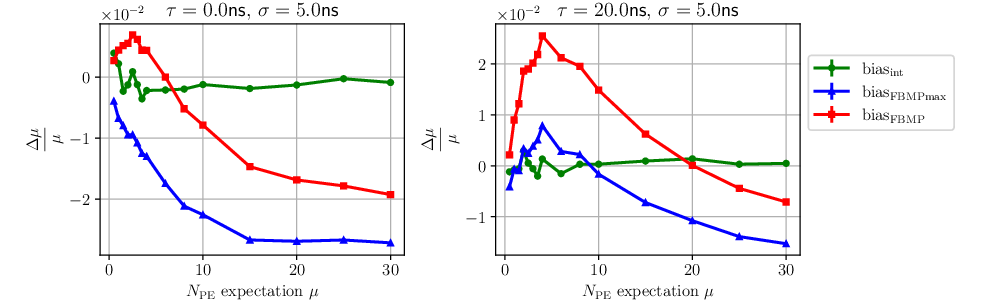
\includegraphics[width=\textwidth]{vs-biasmu-truprior.png}
\end{figure}

\subsection{P-FBMP using different bin width}

\begin{lstlisting}
mu_t = abs(wave.sum() / gmu)
A, wave_r, tlist, t0_t, t0_delta, cha, left_wave, right_wave = wff.initial_params(wave[::wff.nshannon], spe_pre[ent[i]['ChannelID']], Tau, Sigma, gmu, Thres['lucyddm'], p, nsp, nstd, is_t0=True, is_delta=False, n=n, nshannon=1)
mu_t = abs(wave_r.sum() / gmu)
def optit0mu(t0, mu, n, xmmse_star, psy_star, c_star, la):
    ys = np.log(psy_star) - np.log(poisson.pmf(c_star, la)).sum(axis=1)
    ys = np.exp(ys - ys.max()) / np.sum(np.exp(ys - ys.max()))
    t0list = np.arange(t0 - 3 * Sigma, t0 + 3 * Sigma + 1e-6, 0.2)
    mulist = np.arange(max(1e-8, mu - 3 * np.sqrt(mu)), mu + 3 * np.sqrt(mu), 0.1)
    b_mu = [max(1e-8, mu - 5 * np.sqrt(mu)), mu + 5 * np.sqrt(mu)]
    tlist_pan = np.sort(np.unique(np.hstack(np.arange(0, window)[:, None] + np.arange(0, 1, 1 / n))))
    As = np.zeros((len(xmmse_star), len(tlist_pan)))
    As[:, np.isin(tlist_pan, tlist)] = c_star
    assert sum(np.sum(As, axis=0) > 0) > 0

    def likelihood(x):
        a = x[0] * wff.convolve_exp_norm(tlist_pan - x[1], Tau, Sigma) / n + 1e-8 # use tlist_pan not tlist
        li = -special.logsumexp(np.log(poisson.pmf(As, a)).sum(axis=1), b=ys)
        return li

    likemu = np.array([likelihood([mulist[j], t0]) for j in range(len(mulist))])
    liket0 = np.array([likelihood([mu, t0list[j]]) for j in range(len(t0list))])
    mu, t0 = opti.fmin_l_bfgs_b(likelihood, x0=[mulist[likemu.argmin()], t0list[liket0.argmin()]], approx_grad=True, bounds=[b_mu, b_t0], maxfun=50000)[0]
    return mu, t0

truth = pelist[pelist['TriggerNo'] == ent[i]['TriggerNo']]

factor = np.sqrt(np.diag(np.matmul(A.T, A)))
A = np.matmul(A, np.diag(1. / np.sqrt(np.diag(np.matmul(A.T, A)))))
la = mu_t * wff.convolve_exp_norm(tlist - t0_t, Tau, Sigma) / n + 1e-8
xmmse, xmmse_star, psy_star, nu_star, nu_star_bk, T_star, d_tot_i, d_max_i, num_i = wff.fbmpr_fxn_reduced(wave_r, A, la, spe_pre[cid]['std'] ** 2, (gsigma * factor / gmu) ** 2, factor, len(la), stop=5, truth=truth, i=i, left=left_wave, right=right_wave, tlist=tlist, gmu=gmu, para=p)
time_fbmp = time_fbmp + time.time() - time_fbmp_start
c_star = np.zeros_like(xmmse_star).astype(int)
for k in range(len(T_star)):
    t, c = np.unique(T_star[k][xmmse_star[k][T_star[k]] > 0], return_counts=True)
    c_star[k, t] = c
maxindex = 0

xmmse_most = xmmse_star[maxindex]
pet = np.repeat(tlist[xmmse_most > 0], c_star[maxindex][xmmse_most > 0])
cha = np.repeat(xmmse_most[xmmse_most > 0] / factor[xmmse_most > 0] / c_star[maxindex][xmmse_most > 0], c_star[maxindex][xmmse_most > 0])

mu, t0 = optit0mu(t0_t, mu_t, n, xmmse_star, psy_star, c_star, la)
mu_i, t0_i = optit0mu(t0_t, mu_t, n, xmmse_most[None, :], np.array([1]), c_star[maxindex][None, :], la)
\end{lstlisting}

Motivation: to demonstrate the bin width's influence on $\mu$ bias. 

Progress: $1/n$ is the bin width, $n=\{1,2,5\}$

\begin{figure}[H]
    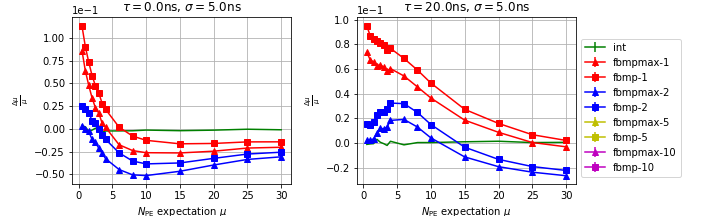
\includegraphics[width=\textwidth]{vs-biasmu-bin.png}
\end{figure}

\subsection{$N_{PE}$ estimation in one bin}

\begin{lstlisting}
def getm(i, p):
    N = 10000
    bias = np.empty(N)
    np.random.seed(i)
    Mu = 10
    gmu = 160
    gsigma = 40
    npan = np.arange(1, 50)
    for i in range(N):
        n = poisson.ppf(1 - uniform.rvs(scale=1-poisson.cdf(0, Mu), size=1), Mu).astype(int)
        cha = norm.ppf(1 - uniform.rvs(scale=1-norm.cdf(0, loc=gmu, scale=gsigma), size=n), loc=gmu, scale=gsigma)
        cha = cha.sum()
        if p:
            weight = poisson.pmf(npan, Mu) * norm.pdf(cha, loc=gmu * npan, scale=gsigma * np.sqrt(npan))
        else:
            weight = norm.pdf(cha, loc=gmu * npan, scale=gsigma * np.sqrt(npan))
        weight = weight / weight.sum()
        bias[i] = np.sum(npan * weight) - n
    m = bias.mean()
    return m
slices = np.arange(1000).T.tolist()
with Pool(100) as pool:
    resultpoisson = np.hstack([pool.starmap(getm, zip(slices, [True] * len(slices)))])
with Pool(100) as pool:
    resultflat = np.hstack([pool.starmap(getm, zip(slices, [False] * len(slices)))])
\end{lstlisting}

Motivation: to estimate bias of $\mu$ based on toy simulation in one bin

Progress: set $\mu$. Sampling: $n\sim\mathrm{Poisson}(n|\mu)$, $q_i\sim\mathrm{Gaussian}(q_i|1,\sigma_q^2),i=\{1,2,\cdots,n\}$, $Q=\sum_i q_i$. Estimation: $p(n|Q) = \frac{\mathrm{Poisson}(n|\mu) \cdot \mathrm{Gaussian}(Q|n,n\sigma_q^2)}{\sum_{j=1}^n \mathrm{Poisson}(j|\mu) \cdot \mathrm{Gaussian}(Q|j,j\sigma_q^2)}$ or $p(n|Q) = \frac{\mathrm{Gaussian}(Q|n,n\sigma_q^2)}{\sum_{j=1}^n \mathrm{Gaussian}(Q|j,j\sigma_q^2)}$

Result: when using Poisson prior, there is \textbf{no} bias, when using flat prior, there is bias. 

\begin{figure}[H]
    \centering
    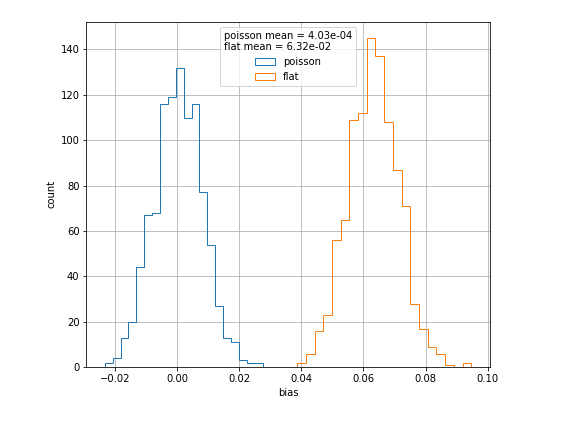
\includegraphics[width=0.5\textwidth]{onebinbias.png}
\end{figure}

\subsection{$N_{PE}$ estimation based on toy simulation}

\begin{lstlisting}
n = 10000
npe = 30
noi = True
if noi:
    std = 1.
else:
    std = 1e-4
window = 200
np.random.seed(0)
wdtp = np.dtype([('No', np.uint32), ('Waveform', np.float, window)])
waves = np.empty(n).astype(wdtp)
tlist = np.repeat(np.array([0, 1, 1]), npe / 3)
sams = [np.vstack((tlist, wff.charge(npe, gmu=gmu, gsigma=gsigma, thres=0))).T for i in range(n)]
pan = np.arange(0, window)
t0 = 0.5
for i in tqdm(range(n)):
    wave = np.sum([np.where(pan > sams[i][j, 0], wff.spe(pan - sams[i][j, 0], tau=p[0], sigma=p[1], A=p[2]) * sams[i][j, 1] / gmu, 0) for j in range(len(sams[i]))], axis=0)
    if noi:
        wave = wave + np.random.normal(0, std, size=window)
    waves[i]['Waveform'] = wave
waves['No'] = np.arange(n).astype(np.uint32)
sdtp = np.dtype([('No', np.uint32), ('HitPosInWindow', np.float64), ('Charge', np.float64)])
pelist = np.empty(sum([len(sams[i]) for i in range(n)])).astype(sdtp)
pelist['No'] = np.repeat(np.arange(n), [len(sams[i]) for i in range(n)]).astype(np.uint32)
pelist['HitPosInWindow'] = np.hstack([sams[i][:, 0] for i in range(n)])
pelist['Charge'] = np.hstack([sams[i][:, 1] for i in range(n)])
mu = np.empty(n)
for i in tqdm(range(n)):
    wave = waves[i]['Waveform'].astype(np.float64) * spe_pre[0]['epulse']
    truth = pelist[pelist['No'] == waves[i]['No']]
    tlist = np.unique(truth['HitPosInWindow'])

    t_auto = np.arange(0, window)[:, None] - tlist
    A = p[2] * np.exp(-1 / 2 * (np.log((t_auto + np.abs(t_auto)) / p[0] / 2) / p[1]) ** 2)
    mu_t = npe
    factor = np.sqrt(np.diag(np.matmul(A.T, A)))
    A = np.matmul(A, np.diag(1. / np.sqrt(np.diag(np.matmul(A.T, A)))))
    la = mu_t * np.array([1, 2]) / 3
    
    xmmse, xmmse_star, psy_star, nu_star, nu_star_bk, T_star, d_tot_i, d_max_i, num_i = wff.fbmpr_fxn_reduced(wave, A, la, std ** 2, (gsigma * factor / gmu) ** 2, factor, len(la), stop=5)
    
    c_star = np.zeros_like(xmmse_star).astype(int)
    for k in range(len(T_star)):
        t, c = np.unique(T_star[k][xmmse_star[k][T_star[k]] > 0], return_counts=True)
        c_star[k, t] = c

    mu[i] = np.average(c_star.sum(axis=1), weights=psy_star)
\end{lstlisting}

Motivation: try to understand the relation between convolution process and bias

Progress: there is no $\mu$, set $N_{PE}$ as 30, set \textit{HitPosInWindow} to $[0, 1]$, set time profile prior as $[1/3, 2/3]$, sample \textit{Charge}. Use FBMP to generate posterior distribution of $N_{PE}$. 

Result: there is \textbf{no} bias on this configuration

\begin{figure}[H]
    \centering
    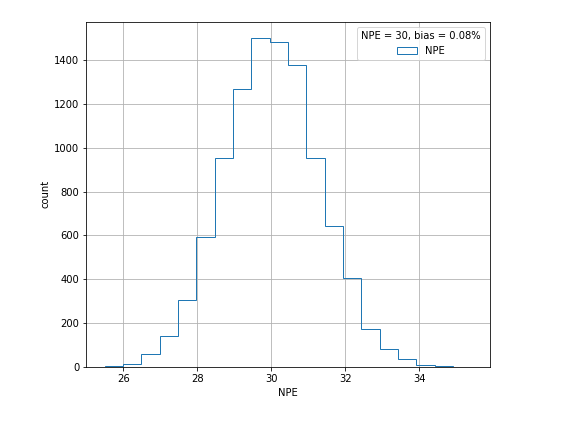
\includegraphics[width=0.5\textwidth]{toybias.png}
\end{figure}

\subsection{Influence of lucyddm \texttt{tlist} initialization on $\mu$ bias}

\begin{lstlisting}
n = 2
A, wave_r, tlist, t0_t, t0_delta, cha, left_wave, right_wave = wff.initial_params(wave[::wff.nshannon], spe_pre[ent[i]['ChannelID']], Tau, Sigma, gmu, Thres['lucyddm'], p, nsp, nstd, is_t0=True, is_delta=False, n=n, nshannon=1)

truth = pelist[pelist['TriggerNo'] == ent[i]['TriggerNo']]

c_star_truth = np.sum([np.where(tlist - 0.5 / n < truth['HitPosInWindow'][j], 1, 0) * np.where(tlist + 0.5 / n > truth['HitPosInWindow'][j], 1, 0) for j in range(len(truth))], axis=0)

mu = c_star_truth.sum()
t0 = t0_t
\end{lstlisting}

Motivation: to test the influence of lucyddm time bin initialization on $\mu$ bias

Progress: lucyddm initialization, estimate $\mu$ as number of truth \textit{HitPosInWindow} in \texttt{tlist}

Result: there is \textbf{no} bias from lucyddm \texttt{tlist} initialization

\begin{figure}[H]
    \centering
    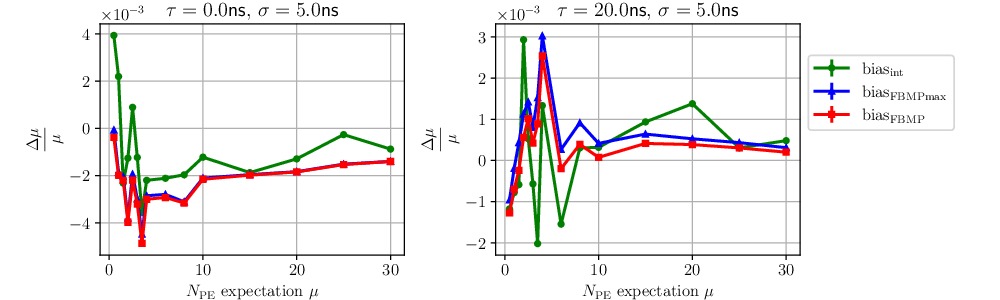
\includegraphics[width=\textwidth]{vs-biasmu-lucyddmtlist.png}
\end{figure}

\subsection{Influence of lucyddm \texttt{wave\_r} initialization on $\mu$ bias}

\begin{lstlisting}
mu_t = abs(wave.sum() / gmu)
n = 2
A, wave_r, tlist, t0_t, t0_delta, cha, left_wave, right_wave = wff.initial_params(wave[::wff.nshannon], spe_pre[ent[i]['ChannelID']], Tau, Sigma, gmu, Thres['lucyddm'], p, nsp, nstd, is_t0=True, is_delta=False, n=n, nshannon=1)
mu_t = abs(wave_r.sum() / gmu)
mu = mu_t
t0 = t0_t
\end{lstlisting}

Motivation: to test the influence of waveform cut in lucyddm initialization on $\mu$ bias

Progress: lucyddm initialization, estimate $\mu$ as number of integral of truncated waveform \texttt{wave\_r}

Result: there is \textbf{no} bias from lucyddm waveform cut initialization

\begin{figure}[H]
    \centering
    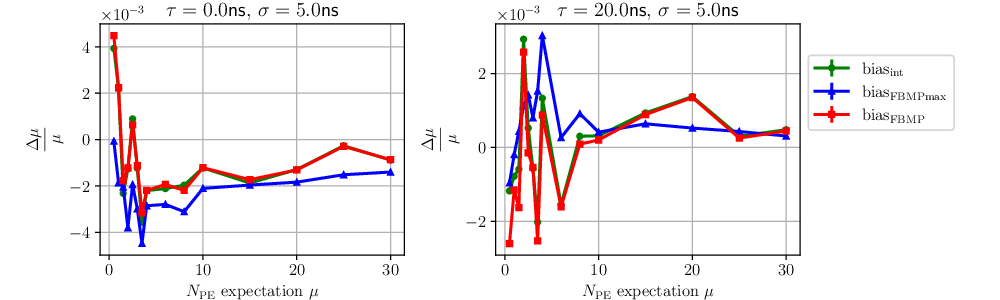
\includegraphics[width=\textwidth]{vs-biasmu-lucyddmwave.png}
\end{figure}

\subsection{Iterative P-FBMP}

\begin{lstlisting}
mu_t = abs(wave.sum() / gmu)
if Tau > 10:
    n = min(math.ceil(20 / mu_t), 5)
else:
    n = min(math.ceil(4 / mu_t), 3)
A, wave_r, tlist, t0_t, t0_delta, cha, left_wave, right_wave = wff.initial_params(wave[::wff.nshannon], spe_pre[ent[i]['ChannelID']], Tau, Sigma, gmu, Thres['lucyddm'], p, nsp, nstd, is_t0=True, is_delta=False, n=n, nshannon=1)
mu_t = abs(wave_r.sum() / gmu)
def optit0mu(t0, mu, n, xmmse_star, psy_star, c_star, la):
    ys = np.log(psy_star) - np.log(poisson.pmf(c_star, la)).sum(axis=1)
    ys = np.exp(ys - ys.max()) / np.sum(np.exp(ys - ys.max()))
    t0list = np.arange(t0 - 3 * Sigma, t0 + 3 * Sigma + 1e-6, 0.2)
    mulist = np.arange(max(1e-8, mu - 3 * np.sqrt(mu)), mu + 3 * np.sqrt(mu), 0.1)
    b_mu = [max(1e-8, mu - 5 * np.sqrt(mu)), mu + 5 * np.sqrt(mu)]
    tlist_pan = np.sort(np.unique(np.hstack(np.arange(0, window)[:, None] + np.arange(0, 1, 1 / n))))
    As = np.zeros((len(xmmse_star), len(tlist_pan)))
    As[:, np.isin(tlist_pan, tlist)] = c_star
    assert sum(np.sum(As, axis=0) > 0) > 0

    def likelihood(x):
        a = x[0] * wff.convolve_exp_norm(tlist_pan - x[1], Tau, Sigma) / n + 1e-8 # use tlist_pan not tlist
        li = -special.logsumexp(np.log(poisson.pmf(As, a)).sum(axis=1), b=ys)
        return li

    likemu = np.array([likelihood([mulist[j], t0]) for j in range(len(mulist))])
    liket0 = np.array([likelihood([mu, t0list[j]]) for j in range(len(t0list))])
    mu, t0 = opti.fmin_l_bfgs_b(likelihood, x0=[mulist[likemu.argmin()], t0list[liket0.argmin()]], approx_grad=True, bounds=[b_mu, b_t0], maxfun=50000)[0]
    return mu, t0

truth = pelist[pelist['TriggerNo'] == ent[i]['TriggerNo']]
time_fbmp_start = time.time()
factor = np.sqrt(np.diag(np.matmul(A.T, A)).mean())
A = np.matmul(A, np.diag(1. / np.sqrt(np.diag(np.matmul(A.T, A)))))

t0_bk = np.inf
mu_bk = np.inf
iterc_i = 0
while abs(mu_bk - mu_t) > 1e-3 or abs(t0_bk - t0_t) > 1e-3:
    iterc_i += 1
    t0_bk = t0_t
    mu_bk = mu_t
    la = mu_t * wff.convolve_exp_norm(tlist - t0_t, Tau, Sigma) / n + 1e-8
    xmmse, xmmse_star, psy_star, nu_star, nu_star_bk, T_star, d_tot_i, d_max_i, num_i = wff.fbmpr_fxn_reduced(wave_r, A, la, spe_pre[cid]['std'] ** 2, (gsigma * factor / gmu) ** 2, factor, len(la), stop=5, truth=truth, i=i, left=left_wave, right=right_wave, tlist=tlist, gmu=gmu, para=p)
    time_fbmp = time_fbmp + time.time() - time_fbmp_start
    c_star = np.zeros_like(xmmse_star).astype(int)
    for k in range(len(T_star)):
        t, c = np.unique(T_star[k][xmmse_star[k][T_star[k]] > 0], return_counts=True)
        c_star[k, t] = c

    mu_t, t0_t = optit0mu(t0_t, mu_t, n, xmmse_star, psy_star, c_star, la)
    if iterc_i >= 10:
        break

mu = mu_t
t0 = t0_t
mu_i, t0_i = optit0mu(t0_t, mu_t, n, xmmse_most[None, :], np.array([1]), c_star[maxindex][None, :], la)
\end{lstlisting}

Motivation: demonstrate whether iteration can reduce $\mu$ bias

Progress: set $\mu=10$ to save time, iteration after FBMP sampling and fitting until $\mu$ and $t_0$ are stable

Result: iteration can \textbf{not} reduce $\mu$ bias

\begin{figure}[H]
    \centering
    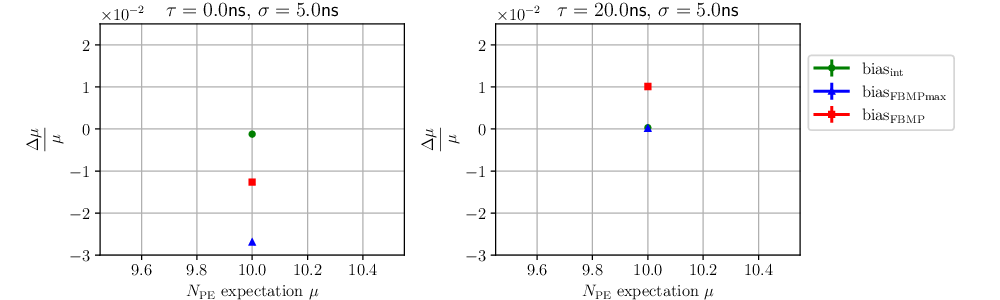
\includegraphics[width=\textwidth]{vs-biasmu-iter.png}
\end{figure}

\subsection{Waveform simulation with fixed \textit{HitPosInWindow}}

Waveform simulation:

\begin{lstlisting}
np.random.seed(a0 + round(Tau + Sigma))
npe = poisson.ppf(1 - uniform.rvs(scale=1-poisson.cdf(0, mu), size=a1 - a0), mu).astype(int)
t0 = np.random.uniform(100., 500., size=a1 - a0)
sams = [np.vstack((np.arange(npe[i]) + t0[i], wff.charge(npe[i], gmu=gmu, gsigma=gsigma, thres=0))).T for i in range(a1 - a0)]
wdtp = np.dtype([('TriggerNo', np.uint32), ('ChannelID', np.uint32), ('Waveform', np.float, window * wff.nshannon)])
waves = np.empty(a1 - a0).astype(wdtp)
pan = np.arange(0, window, 1 / wff.nshannon)
for i in range(a1 - a0):
    wave = np.sum([np.where(pan > sams[i][j, 0], wff.spe(pan - sams[i][j, 0], tau=p[0], sigma=p[1], A=p[2]) * sams[i][j, 1] / gmu, 0) for j in range(len(sams[i]))], axis=0)
    if args.noi:
        wave = wave + np.random.normal(0, std, size=window * wff.nshannon)
    waves[i]['Waveform'] = wave
tdtp = np.dtype([('TriggerNo', np.uint32), ('ChannelID', np.uint32), ('T0', np.float64)])
t = np.empty(a1 - a0).astype(tdtp)
t['TriggerNo'] = np.arange(a0, a1).astype(np.uint32)
t['T0'] = t0
t['ChannelID'] = 0
waves['TriggerNo'] = np.arange(a0, a1).astype(np.uint32)
waves['ChannelID'] = 0
sdtp = np.dtype([('TriggerNo', np.uint32), ('PMTId', np.uint32), ('HitPosInWindow', np.float64), ('Charge', np.float64)])
pelist = np.empty(sum([len(sams[i]) for i in range(a1 - a0)])).astype(sdtp)
pelist['TriggerNo'] = np.repeat(np.arange(a0, a1), [len(sams[i]) for i in range(a1 - a0)]).astype(np.uint32)
pelist['PMTId'] = 0
pelist['HitPosInWindow'] = np.hstack([sams[i][:, 0] for i in range(a1 - a0)])
pelist['Charge'] = np.hstack([sams[i][:, 1] for i in range(a1 - a0)])
\end{lstlisting}

P-FBMP:

\begin{lstlisting}
mu_t = abs(wave.sum() / gmu)
if Tau > 10:
    n = min(math.ceil(20 / mu_t), 5)
else:
    n = min(math.ceil(4 / mu_t), 3)
A, wave_r, tlist, t0_t, t0_delta, cha, left_wave, right_wave = wff.initial_params(wave[::wff.nshannon], spe_pre[ent[i]['ChannelID']], Tau, Sigma, gmu, Thres['lucyddm'], p, nsp, nstd, is_t0=True, is_delta=False, n=n, nshannon=1)

truth = pelist[pelist['TriggerNo'] == ent[i]['TriggerNo']]

tlist = truth['HitPosInWindow'][truth['HitPosInWindow'] < right_wave - 1]
if len(tlist) == 0:
    tlist = np.array([300])
t_auto = (np.arange(left_wave, right_wave) / wff.nshannon)[:, None] - tlist
A = p[2] * np.exp(-1 / 2 * (np.log((t_auto + np.abs(t_auto)) / p[0] / 2) / p[1]) ** 2)

t0_t = t0_truth[i]['T0']
mu_t = len(truth)
factor = np.sqrt(np.diag(np.matmul(A.T, A)))
A = np.matmul(A, np.diag(1. / np.sqrt(np.diag(np.matmul(A.T, A)))))
la = mu_t * np.ones(len(tlist)) / len(tlist)
xmmse, xmmse_star, psy_star, nu_star, nu_star_bk, T_star, d_tot_i, d_max_i, num_i = wff.fbmpr_fxn_reduced(wave_r, A, la, spe_pre[cid]['std'] ** 2, (gsigma * factor / gmu) ** 2, factor, len(la), stop=5, truth=truth, i=i, left=left_wave, right=right_wave, tlist=tlist, gmu=gmu, para=p)
time_fbmp = time_fbmp + time.time() - time_fbmp_start
c_star = np.zeros_like(xmmse_star).astype(int)
for k in range(len(T_star)):
    t, c = np.unique(T_star[k][xmmse_star[k][T_star[k]] > 0], return_counts=True)
    c_star[k, t] = c
maxindex = 0

xmmse_most = xmmse_star[maxindex]
pet = np.repeat(tlist[xmmse_most > 0], c_star[maxindex][xmmse_most > 0])
cha = np.repeat(xmmse_most[xmmse_most > 0] / factor[xmmse_most > 0] / c_star[maxindex][xmmse_most > 0], c_star[maxindex][xmmse_most > 0])

mu = np.average(c_star.sum(axis=1), weights=psy_star)
t0 = t0_t
mu_i = len(cha)
t0_i = t0_t
\end{lstlisting}

Motivation: to further reduce the influence of binning

Progress: when PE number is $N_{PE}$, set \textit{HitPosInWindow} relatively (to $t_0$) $\{0,1,\cdots,N_{PE}-1\}$, sample \textit{Charge} then P-FBMP process with truth prior. 

Result: there is still bias with fixed \textit{HitPosInWindow}

\begin{figure}[H]
    \centering
    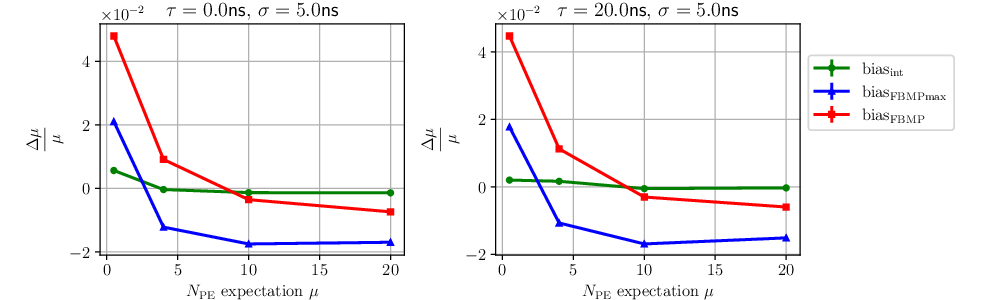
\includegraphics[width=\textwidth]{vs-biasmu-fixtlist.png}
\end{figure}

\subsection{Waveform simulation with fixed \textit{HitPosInWindow} \textbf{without} truth prior}

Waveform simulation:

\begin{lstlisting}
sams = [np.vstack((np.arange(npe[i]) + t0[i], wff.charge(npe[i], gmu=gmu, gsigma=gsigma, thres=0))).T for i in range(a1 - a0)]
\end{lstlisting}

P-FBMP:

\begin{lstlisting}
    def fbmpr_fxn_reduced(y, A, p1, sig2w, sig2s, mus, D, stop=0, truth=None, i=None, left=None, right=None, tlist=None, gmu=None, para=None, prior=True):
    '''
    p1: prior probability for each bin.
    sig2w: variance of white noise.
    sig2s: variance of signal x_i.
    mus: mean of signal x_i.
    '''
    # Only for multi-gaussian with arithmetic sequence of mu and sigma
    M, N = A.shape

    p = 1 - poisson.pmf(0, p1).mean()
    # Eq. (25)
    if prior:
        nu_true_mean = -M / 2 - M / 2 * np.log(sig2w) - p * N / 2 * np.log(sig2s / sig2w + 1) - M / 2 * np.log(2 * np.pi) + N * np.log(1 - p) + p * N * np.log(p / (1 - p))
        nu_true_stdv = np.sqrt(M / 2 + N * p * (1 - p) * (np.log(p / (1 - p)) - np.log(sig2s / sig2w + 1) / 2) ** 2)
    else:
        nu_true_mean = -M / 2 - M / 2 * np.log(sig2w) - p * N / 2 * np.log(sig2s / sig2w + 1) - M / 2 * np.log(2 * np.pi)
        nu_true_stdv = np.sqrt(M / 2 + N * p * (1 - p) * (np.log(sig2s / sig2w + 1) / 2) ** 2)
    nu_stop = (nu_true_mean + stop * nu_true_stdv).max()

    psy_thresh = 1e-4
    # upper limit of number of PEs.
    P = max(math.ceil(min(M, p1.sum() + 3 * np.sqrt(p1.sum()))), 1)

    T = np.full((P, D), 0)
    nu = np.full((P, D), -np.inf)
    xmmse = np.zeros((P, D, N))
    cc = np.zeros((P, D, N))
    d_tot = D

    # nu_root: nu for all s_n=0.
    if prior:
        nu_root = -0.5 * np.linalg.norm(y) ** 2 / sig2w - 0.5 * M * np.log(2 * np.pi) - 0.5 * M * np.log(sig2w) + np.log(poisson.pmf(0, p1)).sum()
    else:
        nu_root = -0.5 * np.linalg.norm(y) ** 2 / sig2w - 0.5 * M * np.log(2 * np.pi) - 0.5 * M * np.log(sig2w)
    # Eq. (29)
    cx_root = A / sig2w
    # Eq. (30) sig2s = 1 sigma^2 - 0 sigma^2
    betaxt_root = sig2s / (1 + sig2s * np.einsum('ij,ij->j', A, cx_root, optimize=True))
    # Eq. (31)
    if prior:
        nuxt_root = nu_root + 0.5 * (betaxt_root * (y @ cx_root + mus / sig2s) ** 2  - mus ** 2 / sig2s + np.log(betaxt_root / sig2s)) + np.log(poisson.pmf(1, p1) / poisson.pmf(0, p1))
    else:
        nuxt_root = nu_root + 0.5 * (betaxt_root * (y @ cx_root + mus / sig2s) ** 2  - mus ** 2 / sig2s + np.log(betaxt_root / sig2s))
    pan_root = np.zeros(N)

    # Repeated Greedy Search
    for d in range(D):
        nuxt = nuxt_root.copy()
        z = y.copy()
        cx = cx_root.copy()
        betaxt = betaxt_root.copy()
        pan = pan_root.copy()
        for p in range(P):
            # look for duplicates of nu and nuxt, set to -inf.
            # only inspect the same number of PEs in Row p.
            nuxtshadow = np.where(np.sum(np.abs(nuxt - nu[p:(p+1), :d].T) < 1e-4, axis=0), -np.inf, nuxt)
            nustar = max(nuxtshadow)
            istar = np.argmax(nuxtshadow)
            nu[p, d] = nustar
            T[p, d] = istar
            pan[istar] += 1
            # Eq. (33)
            cx -= np.einsum('n,m,mp->np', betaxt[istar] * cx[:, istar], cx[:, istar], A, optimize=True)

            # Eq. (34)
            z -= A[:, istar] * mus[istar]
            assist = np.zeros(N)
            t, c = np.unique(T[:p+1, d], return_counts=True)
            assist[t] = mus[t] * c + sig2s[t] * c * np.dot(z, cx[:, t])
            cc[p, d][t] = c
            xmmse[p, d] = assist

            # Eq. (30)
            betaxt = sig2s / (1 + sig2s * np.sum(A * cx, axis=0))
            # Eq. (31)
            if prior:
                nuxt = nustar + 0.5 * (betaxt * (z @ cx + mus / sig2s) ** 2 - mus ** 2 / sig2s + np.log(betaxt / sig2s)) + np.log(poisson.pmf(pan + 1, mu=p1) / poisson.pmf(pan, mu=p1))
            else:
                nuxt = nustar + 0.5 * (betaxt * (z @ cx + mus / sig2s) ** 2 - mus ** 2 / sig2s + np.log(betaxt / sig2s))
            # nuxt[t] = -np.inf

        if max(nu[:, d]) > nu_stop:
            d_tot = d + 1
            break
    nu_bk = nu[:, :d_tot].copy()
    nu = nu[:, :d_tot].T.flatten()

    indx = np.argsort(nu)[::-1]
    d_max = math.floor(indx[0] // P) + 1
    num = min(math.ceil(np.sum(nu > nu.max() + np.log(psy_thresh))), d_tot * P)
    nu_star = nu[indx[:num]]
    nu_star_bk = nu_bk.T.flatten()[indx[:num]]
    # psy_star = np.exp(nu_star - nu.max()) / np.sum(np.exp(nu_star - nu.max()))
    T_star = [np.sort(T[:(indx[k] % P) + 1, indx[k] // P]) for k in range(num)]
    xmmse_star = np.empty((num, N))
    for k in range(num):
        xmmse_star[k] = xmmse[indx[k] % P, indx[k] // P]

    psy_star = np.exp(nu_star - nu.max()) / np.sum(np.exp(nu_star - nu.max()))

    xmmse = np.average(xmmse_star, weights=psy_star, axis=0)

    return xmmse, xmmse_star, psy_star, nu_star, nu_star_bk, T_star, d_tot, d_max, num
\end{lstlisting}

\begin{lstlisting}
prior = False
truth = pelist[pelist['TriggerNo'] == ent[i]['TriggerNo']]

tlist = truth['HitPosInWindow'][truth['HitPosInWindow'] < right_wave - 1]
if len(tlist) == 0:
    tlist = np.array([300])
t_auto = (np.arange(left_wave, right_wave) / wff.nshannon)[:, None] - tlist
A = p[2] * np.exp(-1 / 2 * (np.log((t_auto + np.abs(t_auto)) / p[0] / 2) / p[1]) ** 2)

t0_t = t0_truth[i]['T0']
mu_t = len(truth)
factor = np.sqrt(np.diag(np.matmul(A.T, A)))
A = A / factor
la = mu_t * np.ones(len(tlist)) / len(tlist)
xmmse, xmmse_star, psy_star, nu_star, nu_star_bk, T_star, d_tot_i, d_max_i, num_i = wff.fbmpr_fxn_reduced(wave_r, A, la, spe_pre[cid]['std'] ** 2, (gsigma * factor / gmu) ** 2, factor, len(la), stop=5, truth=truth, i=i, left=left_wave, right=right_wave, tlist=tlist, gmu=gmu, para=p, prior=prior)

mu = np.average(c_star.sum(axis=1), weights=psy_star)
t0 = t0_t
mu_i = len(cha)
t0_i = t0_t
\end{lstlisting}

Motivation: to further reduce the influence of prior

Progress: set \textit{HitPosInWindow} relatively (to $t_0$) $\{0,1,\cdots,N_{PE}-1\}$, P-FBMP process \textbf{without} truth prior. 

Result: all biases \textbf{are larger} than 0

\begin{figure}[H]
    \centering
    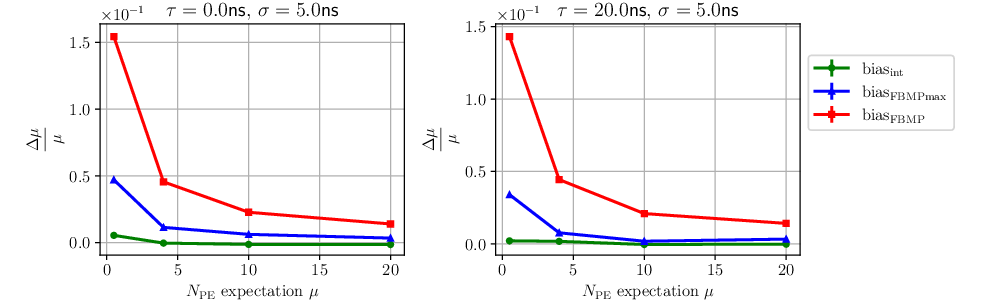
\includegraphics[width=\textwidth]{vs-biasmu-fixtlistnoprior.png}
\end{figure}

\section{Theory}

\subsection{Why bias}

\subsubsection{Model}

\begin{equation}
\begin{aligned}
    \left.
    \begin{bmatrix}
        \bm{w} \\
        \bm{q}'
    \end{bmatrix}
    \right\vert\bm{z}
    &\sim \mathrm{Normal}\left(
    \begin{bmatrix}
        \bm{V}_\mathrm{PE}\bm{z} \\
        \bm{z}
    \end{bmatrix}, 
    \begin{bmatrix}
        \bm{\Sigma} & \bm{V}_\mathrm{PE}\bm{Z} \\
        \bm{Z}\bm{V}_\mathrm{PE}^\intercal & \bm{Z}
    \end{bmatrix}
    \right) \\
    \bm{\Sigma} &= \bm{V}_\mathrm{PE}\bm{Z}\bm{V}_\mathrm{PE}^\intercal+\sigma_\epsilon^2\bm{I}_M 
\end{aligned}
\end{equation}

\begin{equation}
\begin{aligned}
    \nu =& \log[p(\bm{w},\bm{z})] = \log[p(\bm{w}|\bm{z})p(\bm{z})] \\
    =& -\frac{1}{2}(\bm{w}-\bm{V}_\mathrm{PE}\bm{z})^\intercal\bm{\Sigma}^{-1}(\bm{w}-\bm{V}_\mathrm{PE}\bm{z})-\frac{1}{2}\log\det\bm{\Sigma}-\frac{N}{2}\log2\pi \\
    & +\sum_{i}\log{\mathrm{Poisson}(z_i,p_i)}
\end{aligned}
\end{equation}

\subsubsection{Simplification}

\begin{itemize}
    \item Poisson $\rightarrow$ Bernoulli, $z_i=0,\bm{Z}_{ii}=0$ or $z_i=1,\bm{Z}_{ii}=\sigma^2$
    \item SPE $\rightarrow$ delta SPE, $\bm{V}_{PE}=\begin{bmatrix}
        \bm{I} \\
        \bm{O}
    \end{bmatrix}$, $w_i\sim \mathrm{Normal}(1,\sigma^2+\sigma_\epsilon^2)$
    \item flat prior, $\begin{cases}
        \lambda & \text{ if } z_i=1 \\ 
        1-\lambda & \text{ if } z_i=0 
    \end{cases}$
\end{itemize}

\subsubsection{Evaluation}

for a certain $(\bm{w}, \bm{z})$, let $K=\{i|z_i=1\}$, $|K|=n$

\begin{align}
    \bm{\Sigma} &= \begin{bmatrix}
        \bm{Z} & \bm{O} \\
        \bm{O} & \bm{O}
    \end{bmatrix} + \sigma_\epsilon^2\bm{I}_M \\
    \det\bm{\Sigma} &= \Pi_i (z_i\sigma^2+\sigma_\epsilon^2) \\
    \bm{\Sigma}_{ij}^{-1} &= \begin{cases}
        \frac{1}{z_i\sigma^2+\sigma_\epsilon^2} & \text{ if }  i=j \\ 
        0 & \text{ if }  i\neq j 
    \end{cases}
\end{align}

Thus, 

\begin{align}
    -2\nu =& \sum_{i\in K}\frac{(w_i - 1)^2}{\sigma^2+\sigma_\epsilon^2} + \sum_{i\in \bar{K}}\frac{w_i^2}{\sigma_\epsilon^2} \\ 
    +& n\log(\sigma^2+\sigma_\epsilon^2) + (N-n)\log\sigma_\epsilon^2 \\
    -& 2n\log\lambda - 2(N-n)\log(1-\lambda)
\end{align}

Additionally, 

\begin{align}
    \sum_{i\in K}\frac{(w_i - 1)^2}{\sigma^2+\sigma_\epsilon^2} &\sim \chi^2(n) \\
    \frac{w_i^2}{\sigma_\epsilon^2} &= \frac{1}{\sigma_\epsilon^2}((\sigma^2+\sigma_\epsilon^2)\frac{(w_i - 1)^2}{\sigma^2+\sigma_\epsilon^2} + 2(w_i - 1) + 1)
\end{align}

Calculate expectation on distribution of $\bm{w}$ and $\bm{z}$ with $|K|=|\bm{z}|=n$, 

\begin{align}
    -2E(\nu)_n =& n + (N - n)\frac{\sigma^2+\sigma_\epsilon^2}{\sigma_\epsilon^2} + (N - n)\frac{1}{\sigma_\epsilon^2} \\ 
    +& n\log(\sigma^2+\sigma_\epsilon^2) + (N-n)\log\sigma_\epsilon^2 \\
    -& 2n\log\lambda - 2(N-n)\log(1-\lambda)
\end{align}

Thus, 

\begin{align}
    -2D(\nu)_n &= -2E(\nu)_n - (-2E(\nu)_{n-1}) \\ 
    &= 1 - \frac{\sigma^2+\sigma_\epsilon^2}{\sigma_\epsilon^2} - \frac{1}{\sigma_\epsilon^2} \\
    &+ \log(\sigma^2+\sigma_\epsilon^2) - \log\sigma_\epsilon^2 \\
    &- 2\log\lambda + 2\log(1-\lambda)
\end{align}

Remember that $\sigma^2 \gg \sigma_\epsilon^2$ and $\lambda \ll 1$, set $x=\sigma^2/\sigma_\epsilon^2$, then,

\begin{align}
    D(\nu)_n &\approx \frac{1}{2}x - \frac{1}{2}\log x + \log\lambda
\end{align}

while $x \gg 1$, $\frac{1}{2}x - \frac{1}{2}\log x \gg 1$, the sign of $D(\nu)_n$ is defined by the relative magnitude of $\frac{1}{2}x - \frac{1}{2}\log x$ and $\log\lambda$. 

When the time bin is very thin, $\log\lambda \ll 0$, $D(\nu)_n < 0$. When Bernoulli approximation fails, $D(\nu)_n > 0$. 

\subsubsection{Discussion}

While we may reasonably assume $E(\nu)_n$ will be its maximum when $n=N_{PE}$, considering the fact that RGS in FBMP has imperfect ergodicity, the bias will be positive given $D(\nu)_n > 0$ as RGS will \textbf{not} stop immediately when $n=N_{PE}$. Given $D(\nu)_n > 0$, the bias will be negative. 

\section{Ratification}

Induce \textbf{ELBO}. 

\begin{align}
    \mathrm{ELBO} &= E_q(\log(p(\bm{w}|\bm{z}))) - \mathrm{KL}(q|p(\bm{z})) \\
    &= E_q(\log(p(\bm{w}|\bm{z}))) - E_q(\log\frac{q(\bm{z})}{p(\bm{z})}) \\
    &= E_q(\log(p(\bm{w}|\bm{z})p(\bm{z}))) - E_q(\log q(\bm{z})) \\
    &= E_q(\nu) + S_q
\end{align}

where $S$ is entropy. 

Let

\begin{align}
    q(\bm{z})_{\bm{\theta}} &= \begin{cases}
        \frac{f(\bm{\theta},\bm{z})}{\sum_{\bm{z}\in\mathcal{Z}'}f(\bm{\theta},\bm{z})} & \text{ if } \bm{z} \in \mathcal{Z}' \\ 
        0 & \text{ if } \bm{z} \notin \mathcal{Z}'
    \end{cases} \\
    \forall &\bm{z}\in\mathcal{Z}', f(\bm{\theta},\bm{z}) > 0
\end{align}

Noted, $f(\bm{\theta},\bm{z})=\exp{(\nu+g(\bm{\theta},|\bm{z}|))}$ are bad. 

\end{document}